\documentclass[aspectratio=169]{beamer}
\usetheme{Madrid}
\usecolortheme{seahorse}
\usepackage{booktabs}
\usepackage{array}
\usepackage{pgfplots}
\pgfplotsset{compat=1.18}
\title{Static INT8/AWQ Separated Kernel Analysis}
\subtitle{batch=42, separated kernels, 5 rounds x 200 timed iterations}
\author{MoDiff experiment package}
\date{July 1, 2026}

\begin{document}

\begin{frame}
  \titlepage
\end{frame}

\begin{frame}{Scope}
\begin{itemize}
  \item No full-pipeline benchmark results in this deck.
  \item Conv: PyTorch/cuDNN FP16 \texttt{Conv2d} vs current \texttt{OptimizedInt8Conv2d}.
  \item Linear: FP16, current \texttt{int\_gemm}, and AWQ W8A8 backends.
  \item Measurement: 30 warmup iterations, 200 timed iterations, 5 full rounds; tables report median of round medians.
\end{itemize}
\end{frame}

\begin{frame}{Conv2d Implementation Path}
\small
\begin{tabular}{p{0.24\linewidth}p{0.67\linewidth}}
\toprule
Stage & Implementation detail \\
\midrule
Module & \texttt{int8\_optimized.py::OptimizedInt8Conv2d} \\
Input layout & channels-last activation tensor, batch size 42 \\
Weights & per-output-channel symmetric INT8, stored as CUTLASS NHWC filter layout \\
Static quant & \texttt{set\_static\_scale(...)} sets calibrated activation scale and cached inverse scale \\
Benchmark mode & \texttt{modiff\_enabled=False}, \texttt{standard\_output\_fp16=True} \\
Conv kernel call & \texttt{modiff\_cutlass.conv2d\_int8\_fprop\_*} CUTLASS implicit-GEMM conv \\
1x1 special case & \texttt{awq\_fused\_quant\_gemm\_w8a8\_prealloc} over flattened NHWC activations \\
\bottomrule
\end{tabular}
\end{frame}

\begin{frame}{Conv Kernel Sequence}
\small
\begin{tabular}{p{0.20\linewidth}p{0.72\linewidth}}
\toprule
Backend & Kernels called \\
\midrule
FP16 & PyTorch \texttt{nn.Conv2d} dispatches cuDNN/CUTLASS FP16 tensor-core convolution kernels. \\
INT8 3x3 & \texttt{scale\_quantize\_int8} $\rightarrow$ \texttt{conv2d\_int8\_fprop\_dequant\_fp16\_prealloc} or bias/prealloc variant. \\
INT8 1x1 & flatten NHWC to GEMM $M=BHW$ $\rightarrow$ AWQ W8A8 fused quant+GEMM prealloc path. \\
Output boundary & Standard benchmark returns FP16 output to match the LDM baseline wrapper boundary. \\
\bottomrule
\end{tabular}
\end{frame}

\begin{frame}{Linear Implementation Path}
\small
\begin{tabular}{p{0.24\linewidth}p{0.67\linewidth}}
\toprule
Backend & Implementation detail \\
\midrule
FP16 & \texttt{F.linear(x.half(), weight\_fp16, bias)} \\
Current \texttt{int\_gemm} & \texttt{OptimizedInt8Linear(backend='int\_gemm')}; quantize activation, call \texttt{gemm\_w8a8}; square projection shapes may route to AWQ fallback. \\
AWQ & \texttt{backend='awq'}; calls \texttt{awq\_fused\_quant\_gemm\_w8a8} or \texttt{awq\_gemm\_w8a8}. \\
Weights & per-tensor INT8 weight plus FP16 bias; AWQ layout keeps output-major \texttt{weight\_int8\_awq}. \\
Benchmark mode & \texttt{modiff\_enabled=False}, \texttt{standard\_output\_fp16=True}. \\
\bottomrule
\end{tabular}
\end{frame}

\begin{frame}{GEMM Shapes Benchmarked}
\small
\begin{tabular}{lrrr}
\toprule
Index / shape & M & K & N \\
\midrule
{[1]} attn\_proj\_320\_m2688 & 2688 & 320 & 320 \\
{[2]} attn\_proj\_320\_m5376 & 5376 & 320 & 320 \\
{[3]} attn\_proj\_512 & 5376 & 512 & 512 \\
{[4]} attn\_proj\_640\_m2688 & 2688 & 640 & 640 \\
{[5]} ffn\_512\_2048 & 5376 & 512 & 2048 \\
{[6]} ffn\_640\_2560 & 2688 & 640 & 2560 \\
{[7]} large\_2048 & 2048 & 2048 & 2048 \\
{[8]} large\_4096 & 1024 & 4096 & 4096 \\
{[9]} small\_m\_4096 & 128 & 4096 & 4096 \\
\bottomrule
\end{tabular}
\end{frame}

\begin{frame}{Conv Shapes Benchmarked}
\scriptsize
\begin{tabular}{llrrrrr}
\toprule
Index & Shape & B & Cin & H$\times$W & Cout & K \\
\midrule
{[1]} & res\_128\_64 & 42 & 128 & 64$\times$64 & 128 & 3 \\
{[2]} & res\_128\_32 & 42 & 128 & 32$\times$32 & 128 & 3 \\
{[3]} & down\_128\_256\_32 & 42 & 128 & 32$\times$32 & 256 & 3 \\
{[4]} & res\_256\_32 & 42 & 256 & 32$\times$32 & 256 & 3 \\
{[5]} & res\_256\_16 & 42 & 256 & 16$\times$16 & 256 & 3 \\
{[6]} & down\_256\_512\_16 & 42 & 256 & 16$\times$16 & 512 & 3 \\
{[7]} & mid\_512\_8 & 42 & 512 & 8$\times$8 & 512 & 3 \\
{[8]} & up\_512\_256\_16 & 42 & 512 & 16$\times$16 & 256 & 3 \\
{[9]} & up\_256\_128\_32 & 42 & 256 & 32$\times$32 & 128 & 3 \\
{[10]} & up\_128\_64 & 42 & 128 & 64$\times$64 & 128 & 3 \\
{[11]} & pointwise\_320\_16 & 42 & 320 & 16$\times$16 & 320 & 1 \\
\bottomrule
\end{tabular}
\end{frame}

\begin{frame}{Conv Speedup: FP16 / INT8}
\centering
\begin{tikzpicture}
\begin{axis}[
  ybar,
  width=\linewidth,
  height=0.62\textheight,
  ymin=0,
  ymax=1.55,
  ylabel={speedup, FP16 / INT8},
  symbolic x coords={{[1]},{[2]},{[3]},{[4]},{[5]},{[6]},{[7]},{[8]},{[9]},{[10]},{[11]}},
  xtick=data,
  xlabel={conv shape index},
  bar width=8pt,
  nodes near coords,
  nodes near coords style={font=\tiny, /pgf/number format/fixed, /pgf/number format/precision=2},
  grid=major,
  major grid style={draw=gray!20},
]
\addplot+[fill=orange!70, draw=orange!80!black] coordinates {
  ({[1]},0.70) ({[2]},0.73) ({[3]},0.93) ({[4]},0.96) ({[5]},0.94)
  ({[6]},1.12) ({[7]},1.36) ({[8]},0.96) ({[9]},0.70) ({[10]},0.70) ({[11]},0.56)
};
\addplot+[black, dashed, mark=none] coordinates {({[1]},1.0) ({[11]},1.0)};
\end{axis}
\end{tikzpicture}


\end{frame}

\begin{frame}{Conv Latency Table}
\scriptsize
\begin{tabular}{lrrr}
\toprule
Shape & FP16 ms & INT8 ms & FP16/INT8 \\
\midrule
res\_128\_64 & 0.5946 & 0.8555 & 0.70x \\
res\_128\_32 & 0.1708 & 0.2330 & 0.73x \\
down\_128\_256\_32 & 0.3192 & 0.3423 & 0.93x \\
res\_256\_32 & 0.5136 & 0.5349 & 0.96x \\
res\_256\_16 & 0.1354 & 0.1446 & 0.94x \\
down\_256\_512\_16 & 0.2514 & 0.2245 & 1.12x \\
mid\_512\_8 & 0.1340 & 0.0988 & 1.36x \\
up\_512\_256\_16 & 0.2330 & 0.2424 & 0.96x \\
up\_256\_128\_32 & 0.2684 & 0.3812 & 0.70x \\
up\_128\_64 & 0.6022 & 0.8576 & 0.70x \\
pointwise\_320\_16 & 0.0747 & 0.1326 & 0.56x \\
\bottomrule
\end{tabular}
\end{frame}

\begin{frame}{Linear Speedup: Current int\_gemm / AWQ}
\centering
\begin{tikzpicture}
\begin{axis}[
  ybar,
  width=\linewidth,
  height=0.62\textheight,
  ymin=0,
  ymax=7.0,
  ylabel={speedup, int\_gemm / AWQ},
  symbolic x coords={{[1]},{[2]},{[3]},{[4]},{[5]},{[6]},{[7]},{[8]},{[9]}},
  xtick=data,
  xlabel={linear shape index},
  bar width=10pt,
  nodes near coords,
  nodes near coords style={font=\tiny, /pgf/number format/fixed, /pgf/number format/precision=2},
  grid=major,
  major grid style={draw=gray!20},
]
\addplot+[fill=green!55!black, draw=green!35!black] coordinates {
  ({[1]},2.67) ({[2]},2.39) ({[3]},1.03) ({[4]},2.44) ({[5]},6.41)
  ({[6]},5.71) ({[7]},1.00) ({[8]},1.00) ({[9]},0.53)
};
\addplot+[black, dashed, mark=none] coordinates {({[1]},1.0) ({[9]},1.0)};
\end{axis}
\end{tikzpicture}

\end{frame}

\begin{frame}{Linear Latency Table}
\scriptsize
\begin{tabular}{lrrrr}
\toprule
Shape & FP16 ms & int\_gemm ms & AWQ ms & int\_gemm/AWQ \\
\midrule
attn\_proj\_320\_m2688 & 0.0403 & 0.2639 & 0.0989 & 2.67x \\
attn\_proj\_320\_m5376 & 0.0474 & 0.2552 & 0.1067 & 2.39x \\
attn\_proj\_512 & 0.0525 & 0.1176 & 0.1142 & 1.03x \\
attn\_proj\_640\_m2688 & 0.0519 & 0.2550 & 0.1047 & 2.44x \\
ffn\_512\_2048 & 0.1621 & 1.0941 & 0.1706 & 6.41x \\
ffn\_640\_2560 & 0.1074 & 0.7151 & 0.1252 & 5.71x \\
large\_2048 & 0.1771 & 0.1782 & 0.1784 & 1.00x \\
large\_4096 & 0.3514 & 0.2678 & 0.2667 & 1.00x \\
small\_m\_4096 & 0.0804 & 0.2287 & 0.4344 & 0.53x \\
\bottomrule
\end{tabular}
\end{frame}

\begin{frame}{Takeaways}
\begin{itemize}
  \item INT8 conv wins on high-channel smaller-spatial shapes: \texttt{down\_256\_512\_16} and \texttt{mid\_512\_8}.
  \item INT8 conv loses on large-spatial 128-channel shapes and the tested 1x1 pointwise case.
  \item AWQ is consistently better than current \texttt{int\_gemm} for attention/FFN projection shapes, but not for very small M.
  \item The separated-kernel results isolate kernel behavior; they intentionally avoid full-pipeline timing.
\end{itemize}
\end{frame}

\end{document}
